%% METHODS %%%%%%%%%%%%%%%%%%%%%%%%%%%%%%%%%%%%%%%%%%%%%%%%
\section{The automatic state decomposition algorithm}
\label{section:methods}

% TODO:
%  - caption for algorithm flowchart
%  - citation for why conformational averaging is bad

Based on the theory above, we provide a list of practical considerations for an automatic state decomposition algorithm and then present an algorithm that meets the criteria proposed below.
The algorithm operates on an ensemble of molecular dynamics trajectories where conformations (the Cartesian coordinates of all atoms of the macromolecule) have been stored at regular intervals.
In this work, we apply the method to a set of \emph{equilibrium} trajectories at the temperature of interest, but the algorithm can in principle be applied to trajectories generated from \emph{biased} initial conditions, provided the unbiased transition probabilities between regions of configuration space can be computed.
We stress that the algorithm presented here is simply a first attempt at a truly general and automatic algorithm for use with biomacromolecules. 

\subsection{Practical considerations for an automatic state decomposition algorithm.}
\label{section:methods:desiderata}

There are several desirable properties that a state decomposition should possess to be both useful and practical:
\begin{enumerate}
  \item It is not uncommon for simulations conducted on supercomputers such as Blue Gene \cite{fitch:2003a,germain:2005a}, distributed computing platforms such as Folding@Home \cite{pande:2000a,pande:2003a}, or even computer clusters to generate datasets that may contain $10^5$ to $10^7$ configurations in up to $10^4$ trajectories, therefore prohibiting the use of any algorithm with a time complexity greater than $\mathcal{O}(N \log N)$ in the number of configurations.
  \item Molecules may have symmetries under permutation of atoms, such as aromatic rings, the protons on methyl groups, and the oxygens of carboxylate groups that should be accounted for in some way.
  \item The state decomposition algorithm should produce a decomposition for which dynamics appears to be Markovian at the shortest possible lag time $\tau$, so as to produce the most useful model.
  \item The resulting model should not generate so many states so that the elements of the transition matrix will be statistically unreliable.
\end{enumerate}

\subsection{Sketch of the method.}
\label{section:methods:sketch}

\begin{figure}[tb]
  \begin{center}
    \resizebox{3.375in}{!}{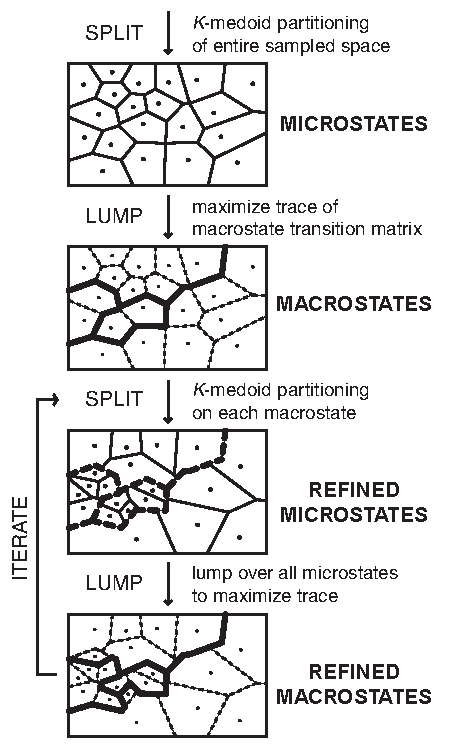
\includegraphics{chapters/automatic-state-decomposition/figures/flowchartsmall.pdf}}    
  \end{center}
  \caption{{\bf Flowchart of the automatic state decomposition algorithm.}}
  \label{figure:methods-flowchart}
\end{figure}

A state decomposition algorithm intended to produce the most \emph{useful} models, as discussed in Section \ref{section:theory:requirements-for-markovian-behavior} above, would generate models that minimize the internal equilibration time $\tau_\mathrm{int}$, the minimum time for which the model behaves in a Markovian fashion.
Unfortunately, $\tau_\mathrm{int}$ is difficult to determine directly, so we are instead forced to identify some surrogate quantity whose maximization will hopefully lead to improved separation between fast intrastate and slow interstate timescales.
Following the approach of Ref.\ \cite{huisinga:2005a}, we define a measure of the \emph{metastability} $Q$ of a partitioning into $L$ \emph{macrostates} as the sum of the self-transition probabilities for a given lag time $\tau$:
\begin{eqnarray}
Q &\equiv& \sum_{i=1}^L T_{ii}(\tau) \label{equation:metastability}
\end{eqnarray}
For $\tau = 0$, $Q = L$, and decays to unity as $\tau$ grows large enough for the self-transition probabilities $T_{ii}$ to reach the equilibrium probabilities of each macrostate.
Poor partitionings into weakly metastable states will result in a small $Q$, as trajectories started in some states will rapidly exit; conversely, good partitionings into strongly metastable states will result in a large $Q$, as trajectories will remain in each macrostate for long times.
In the absence of statistical uncertainty, $Q$ is bounded from above by the sum of the $L$ largest eigenvalues of the true dynamical propagator for the system \cite{huisinga:2005a}.

The goal of our algorithm is to identify a partitioning into $L$ contiguous macrostates that maximizes the metastability $Q$.
While in principle, the boundaries between these macrostates can be varied directly to optimize $Q$, in analogy to variational transition state theory \cite{truhlar:1996a}, a complicated parameterization may be necessary to describe the potentially highly convoluted hypersurfaces separating the states, and $Q$ may have multiple maxima in these parameters.
Instead, we choose an approach based on \emph{splitting} the conformation space into a large number of small contiguous \emph{microstates} and then \emph{lumping} these microstates into macrostates in such a way that maximizes the metastability.
% During this process, we choose some lag time $\tau$ that is less than or equal to the fastest timescale of interest.

This approach is very similar to the approach of Sch\"{u}tte and coworkers described in Ref.\ \cite{schuette:1999a}, but with a substantial difference.
In their work, each degree of freedom of the molecule (such as a torsion angle) is subdivided independently to produce a multidimensional grid.
As the number of states is exponential in the number of degrees of freedom, this approach quickly becomes intractable for macromolecules that possess large numbers of degrees of freedom, even if the sparsity of the transition matrix is taken into account.
Instead, we choose to let the data define the low-dimensional manifold of configuration space accessible to the macromolecule, and we can apply any clustering algorithm that is no worse than $\mathcal{O}(N \log N)$ in the number of configurations to decompose the sampled conformation space into a set of $K$ contiguous microstates.
This step corresponds to the first \emph{split} step in Figure \ref{figure:methods-flowchart}.

Once the conformation space is divided into $K$ microstates, we \emph{lump} the microstates together to produce $L < K$ macrostates with high metastability, $Q$.
This corresponds to the first \emph{lump} step in Figure \ref{figure:methods-flowchart}.  
% As described in Section \ref{section:theory:construction-from-simulation-data}, we can calculate a transition probability matrix for any decomposition of configuration space.
% The \emph{lump} step illustrated in Figure \ref{figure:methods-flowchart} combines the $K$ microstates into $L$ macrostates, calculates the new transition matrix between the macrostates, and chooses a lumping with high metastability.
The difficulty here is that the uncertainty in the metastability of a partitioning can be large if any macrostate contains very few configurations.
Since a macrostate may consist of a single microstate, the microstates must be large enough for the self-transition elements to be statistically well-determined.
%The difficulty here is that if the microstates are too small, the number of observed transitions from each microstate will be small, and the elements of the microstate transition matrix will be dominated by statistical uncertainty.
%To avoid this, the microstates must be large enough for the transition matrix to be well-determined.
This comes at a price: with large microstates, the procedure may have difficulty accurately determining the boundaries between macrostates because the resolution of partitioning is limited by the finite extent of the microstates.
%Additionally, the choice of decomposition into microstates is arbitrary, whereas we would like the state decomposition algorithm to give us the same set of macrostates regardless of how it was initialized.
Additionally, the choice of decomposition into microstates is arbitrary, whereas we would like the state decomposition algorithm to produce equivalent sets of macrostates regardless of how good the initial partitioning was.

To overcome these difficulties, we \emph{iterate} the aforementioned procedure.
After microstates are combined into macrostates, each macrostate is again fragmented into a new set of microstates (the second \emph{split} step in Figure \ref{figure:methods-flowchart}).
The refined set of all microstates is then lumped to form refined macrostates (the second \emph{lump} step in Figure \ref{figure:methods-flowchart}).
In this way, the boundaries between macrostates are iteratively refined, and regions incorrectly lumped in previous iterations may be split off and lumped with the correct macrostate in subsequent iterations.
At convergence, the same set of macrostates will simply be split and lumped back together in the same way --- no further shuffling of conformations between macrostates will occur.

There is unfortunately no unambiguous way to choose the number of states $L$.
If there is a clean separation of timescales, examination of the eigenvalue spectrum of the microstate transition matrix may suggest an appropriate value of $L$ \cite{schuette:2002b}.
In a hierarchical system, there will be many gaps in the eigenvalue spectrum and many of choices of $L$ will lead to good Markovian models of varying complexity.
There is, however, a tradeoff between the number of states and the amount of data needed to obtain a model with the same statistical precision.
It may be necessary to apply the algorithm with multiple choices of $L$ to produce a model sufficient for resolving the timescales of interest.

%In a strongly hierarchical system, where there are several ranges of timescales well-separated from each other, there are many potential choices of $L$ that will lead to good Markovian models.
%In this case, several models of varying complexity can be made.
%For systems without strong separations of timescales, we find that the few fastest timescales are poorly described, but the slowest timescales are generally well-captured, and so $L$ should be chosen somewhat larger than the number of desired states.
%(For a more complete discussion, see [CITE ZIB WORK ON TIMESCALES AND CHOICE OF L].)
%In any case, $L$ must be chosen large enough such that the fastest implied timescales of the model (as revealed by the eigenvalue decomposition of the transition matrix) are comparable to or faster than the timescales of interest.
%Alternatively, $L$ could be chosen to provide a level of complexity of interest.
%Finally, there is a tradeoff between the number of states and the amount of data needed to accurately characterize the transition matrix --- more data will be needed to characterize models with more states, but this does depend on the particular details of the system.

\subsection{Implementation.}
\label{section:methods:implementation}

There are a number of implementation choices to be made in the algorithm given above, and here we briefly summarize and justify our selections.

For the split step, we choose to apply $K$-medoid clustering \cite{hastie:2001a} because of its $\mathcal{O}(KN)$ time complexity (where $K$ can be taken to be constant) and ease of parallelization.
Additionally, $K$-medoid clustering has an advantage over the more popular $K$-means clustering \cite{macqueen:1967} in this application, as it does not require averaging over conformations, which may produce nonsensical constructs when drastically different conformations are included in the average.
Splitting by $K$-medoid clustering is initiated from a random choice of $K$ unique conformations to function as \emph{generators}.
All conformations are assigned to the microstate identified by the generator they are closest to by some distance metric (defined below).
Next, an attempt is made to update the generator of each microstate.
$K$ members of the microstate, drawn at random, are evaluated to see if they reduce the intrastate variance of some distance metric from the generator.
If so, the configuration for which the intrastate variance is minimal is assigned as the new generator.
All conformations are then reassigned to the closest generator, and the process of updating the generators is repeated.
In standard $K$-medoid applications, this procedure is iterated to convergence, but since the purpose of the splitting phase is simply to divide the sampled manifold of configuration space into contiguous states, ensuring that each state is significantly populated, only five iterations of this procedure were used.

For the distance metric, we selected the root-mean squared deviation (RMSD), computed after a minimizing rigid body translation and rotation using the rapid algorithm of Theobald \cite{theobald:2005a}.
In the first splitting iteration, only C$_\alpha$ atoms were used to compute the RMSD due to the expense of having to cluster all conformations in the dataset; in subsequent iterations, all heavy atoms (excepting those indistinguishable by symmetry) were used, as well as sidechain polar hydrogens.
This metric was chosen because it possesses all the qualities of a proper distance metric \cite{steipe:2002a}, accounts for both local similarities between pairs of conformations as well as global ones, and runs in time proportional to the number of atoms, as opposed to a metric such as distance matrix error (DME or dRMSD), which scales as the square of the number of atoms.  
%Atoms related by a symmetry relation are interchangeable in the conformation, so the distance metric shouldn't differentiate these conformations.
In molecules with additional symmetry, the distance metric can be adjusted accordingly.
Our choice of distance metric is not the only one that would suffice; any distance metric which can distinguish between kinetically distinct conformations is sufficient for this algorithm.
For example, backbone RMSD would ignore potentially relevant sidechain kinetics.

Lumping to $L$ states so as to maximize the metastability $Q$ of the macrostates proceeds in two stages.
In the first stage, information on the metastable state structure contained in the slowest eigenvectors \cite{schuette-thesis,huisinga-thesis,deuflhard:2000a,schuette:2002b} is used to construct an initial guess at the optimal lumping.
Because the eigenvectors contain statistical noise, this initial guess may not actually be optimal; because of this, we include a second stage that uses a Monte Carlo simulated annealing (MCSA) optimization algorithm to attempt to further improve the metastability.
Though the MCSA algorithm could in principle be used without the first stage to find optimal lumpings, we find its convergence is greatly accelerated by use of the initial guess.

In the first stage, a transition matrix among microstates is computed (using Eq.\ \ref{equation:transition-element-correlation-functions}) taking advantage of both stationarity and time-reversibility for a short lag time $\tau$, typically the shortest interval at which configurations were stored.
%Each eigenvector, considered in order from largest non-unit eigenvalue to smallest, specifies that a single macrostate is to be further subdivided into two new macrostates.
Motivated by the Perron cluster cluster analysis (PCCA) algorithm of Deuflhard \emph{et al.\ } \cite{deuflhard:2000a}, an initial guess for the optimal lumping of microstates to macrostates is generated using the \emph{left} eigenvectors\footnote{The left eigenvector $\bfm{v}_k$ is simply related to the right eigenvector $\bfm{u}_k$ by $(\bfm{v}_k)_i = p_{\mathrm{eq},i}^{-1} \, (\bfm{u}_k)_i$ \cite{oppenheim:1977a}.} associated with the largest eigenvalues of the microstate transition matrix.
% If we group together microstates with similar left eigenvector components from the set of eigenvectors associated with the longest timescales, these microstates should interconvert on shorter timescales, and therefore the metastability of the partitioning will be high \cite{schuette-thesis,huisinga-thesis,deuflhard:2000a,schuette:2002b}.
We begin by assigning all microstates to a single macrostate.
For each eigenvalue, the corresponding eigenvector contains information about an aggregate transition between the set of microstates with positive eigenvector components and the set with negative components, with a timescale determined by the eigenvalue; equilibration within each set must occur on a faster timescale, provided the eigenvalues are non-degenerate.
We can therefore use this information to identify one macrostate to divide in two.
We select the macrostate with the largest $L_1$ norm of the vector formed from the eigenvector components that belong to that macrostate, after subtracting the mean of this vector, as the state to split.
In Ref.\ \cite{deuflhard:2000a}, the sign structure alone was used to split these sets, but we find it more stable to split about the mean.
This procedure is performed for eigenvectors $k = 2,\ldots,L$ in order, which should correspond to the slowest processes in the system, generating a total of $L$ macrostates.

%However, simply grouping states together based on eigenvector components often did not result in a lumping with maximum metastability $Q$ or preserved timescales.
Due to statistical noise in the eigenvectors and near-degeneracy in the eigenvalues, this procedure does not always result in the lumping with the maximal metastability $Q$.
Therefore, in the second stage, the metastability was maximized using a Monte Carlo simulated annealing (MCSA) algorithm, using the eigenvector-generated lumping as an initial seed.
In each step of the Monte Carlo procedure, a microstate was selected with uniform probability and assigned to a random macrostate.
If this proposed move would leave a macrostate empty or did not change the partitioning, it was rejected immediately.
The proposed partitioning was accepted with probability $\min \{1, e^{\beta \Delta Q} \}$, where the metastability $Q$ of the proposed lumping was rapidly computed by combining elements of the matrix of inter-microstate transition counts.
The effective inverse temperature parameter $\beta$ was set to be equal to the step number, and the MCSA procedure run for 20 000 steps.
Twenty independent MCSA runs were initiated from the initial eigenvector-based partitioning, and the partitioning with the highest metastability sampled in any run was selected to define the lumping into macrostates.

It should be noted that the metastability $Q$ is not the only surrogate that could be optimized in order to produce a useful state decomposition.
Many choices may be possible, especially when one considers the problem of lumping as an attempt to preserve the $L$ longest timescales (determined by the eigenvalues of the transition matrix near unity) present in the microstate transition matrix.
One could choose to maximize the fastest eigenvalue or timescale of the lumped transition matrix, the product of eigenvalues (which would give more weight to faster timescales), or even a weighted sum of the eigenvalues, where the weights might be due to the equilibrium importance of the eigenmode in dynamics or in modeling a process of interest.
Unfortunately, these quantities all necessitate computing some eigenvalues or the determinant of the lumped transition matrix for every proposed lumping to be evaluated by the MCSA algorithm, which would add significant computational burden.
Alternatively, other quantities could be computed from the transition matrix directly, such as the state lifetimes estimated from the self-transition probabilities as $\tau_{L,i} = (1 - T_{ii})^{-1}$.
However, the combination of computational and theoretical convenience makes the use of metastability a natural choice here.

For the remaining iterations, the $K$-medoid clustering is repeated independently on each macrostate.
We set a minimum expected microstate size (estimated by the population of the macrostate divided by $K$) to ensure statistical reliability of the transition probability matrix.
This is set to 100 configurations (unless otherwise noted), though a more useful criteria may be to set a minimum number of statistically independent visits to the state.
Each macrostate is split into a number of states such that the expected microstate population (assuming even division into microstates) is no smaller than this threshold, or a maximum of 10 microstates.
The lumping step is then repeated on all resulting microstates.
The entire procudure of splitting and lumping was repeated for a total of 10 iterations, which for the applications considered here was sufficient for convergence of the slowest timescales.

\subsection{Validation.}
\label{section:methods:validation}

To validate the model, we examine the largest implied timescales as a function of lag time, as computed for the eigenvalues of the transition matrix by Eq.\ \ref{equation:implied-timescales}.
In particular, we attempt to determine the minimum lag time after which the implied timescales appear to be independent of lag time to within the estimated statistical uncertainty (see Section \ref{section:theory:validation}).
To estimate the statistical uncertainty of these implied timescales, we perform a bootstrapping procedure \cite{efron:1979a} on the pool of independent trajectories.
Forty bootstrap samples of a number of trajectories equal to the number of independent trajectories in the dataset pool are generated, drawn with replacement from the pool of trajectories, except for alanine dipeptide, where 100 bootstrap samples were used.
The implied timescales are computed for each sample, and the set of computed timescales is used to estimate a confidence interval.
In figures, uncertainties will always be shown as 68\% symmetric confidence intervals about the mean of the bootstrap sample, while uncertainties in quantities printed as $a \pm b$ will indicate variances about the mean.





